%
% This is a template for a new research paper. For information on this file
% please contact Joe Loughry at Tel. +1 720 277 7800 (time zone GMT minus 7
% hours) or Email: Joe.Loughry@cs.du.edu or mailto:Joe.Loughry@gmail.com
%

\documentclass[conference]{IEEEtran}

\usepackage{cite}

\usepackage[english,british]{babel}
\usepackage{graphicx}
\usepackage[binary-units]{siunitx}
\usepackage[obeyspaces,hyphens]{url}
\newcommand{\URL}[1]{$\langle$\url{#1}$\rangle$}
\usepackage[plainpages=false,pdfpagelabels]{hyperref}
\usepackage{comment}

\hyphenation{op-tical net-works semi-conduc-tor}

% required copyright notice
\IEEEoverridecommandlockouts
\IEEEpubid{\makebox[\columnwidth]{978-1-4673-9698-1/18/\$31.00~\copyright
2018 IEEE \hfill}
\hspace{\columnsep}\makebox[\columnwidth]{ }}

\begin{document}

\title{Optical TEMPEST
}

\author{\IEEEauthorblockN{Joe Loughry}
\IEEEauthorblockA{University of Denver \\
Denver, Colorado 80208 USA \\
Email: joe.loughry@cs.du.edu}}

% I wish IEEEtran would put a date on the title page. I hate it when
% papers don't have dates on them. At least at the bottom there's a tiny
% little `Copyright 2018 IEEE' notice for the reader to find someday.

\maketitle

\begin{abstract}
	Research on optical TEMPEST has exploded since 2002 when the first papers
appeared from widely separated locations within a week of each other. In the
intervening time, vulnerabilities have evolved along with hardware, and
several new threat vectors have appeared. Although the supply chain ecosystem
of Ethernet has reduced the vulnerability of billions of devices through use
of standardised PHY chips, other recent trends including High Frequency
Trading (HFT) in the financial sector, the Internet of Things (IoT), and
inexpensive drones have made it relevant again.

\end{abstract}

\section{Introduction}

Since the publication sixteen years ago of the first two papers on optical
TEMPEST, open source information on security of compromising emanations---and
side channels in general---has exploded. Before the late 1990s, only a
handful of papers had been published in the open literature on the subject of
TEMPEST\footnote{TEMPEST, here, is the U.S.\ National Security Agency (NSA)
code name for `the problem of compromising radiation'---radio frequency (RF)
\emph{or} acoustic, according to the original reference, which was only
declassified in 2007---including both exploitation and control
\cite{NSATempest2007}. Beyond the 1972 definition of TEMPEST, military and
academic researchers have since expanded the spectrum of interest to include
DC, optical, thermal, magnetic, and acceleration side channels.} and the
topic was mostly relegated to the folklore of infosec; the only two
scientific studies of unintentional compromising emanations remained van Eck
\cite{vanEck1985} and Smulders \cite{Smulders1990} although Wright's book
around the same time \cite{Wright1987} described anecdotal reports dating
back to the first world war. But following Kocher's seminal 1996 paper on
side channel attacks \cite{Kocher1996} and Kuhn \& Anderson \cite{Kuhn1998a}
having shown---essentially by adding forward error correction to EMC---that
covert channels were not limited by the system boundary, two papers appeared
within a week of each other on complementary aspects of optical emanations
\cite{Kuhn2002,Loughry2002a}. Since then, the two papers, between them, have
been cited more than 300 times.

\subsection{Organisation}

The first part of this paper is a brief review of the results in the first
paper on optical TEMPEST and a critique of mistakes that were made by one
of the first investigators of the phenomenon, in the methodology, model
building, writing, and follow-up of the earliest research. This is followed
by a survey of ways that later authors have repaired the damage. A cautionary
tale of forgetting lessons learnt in security is rounded out by a description
of some aspects of the the design of a new information security product with
these principles in mind.

\section{The story I never told you before}

Optical TEMPEST was discovered working at a bank. In the raised-floor
computer room on the sixth level of a glass high-rise building in downtown
Seattle, surrounded by other glass high-rises with their own computer rooms
visible at night by the reddish glow of Light Emitting Diode (LED)
indicators, I was working very late. Dial-up modems had not yet gone
completely extinct, \SI{10}{\mega\bit\per\second} Ethernet was increasingly
common on PCs, and leased lines ran everywhere from the computer room to
branch offices, thousands of them. This was the environment where optical
TEMPEST was discovered in 1992. I told my postgraduate professor at Seattle
U.\ about it. Cautious experiments were performed. A literature survey was
quietly done to see if anyone had ever noticed it before, and the National
Computer Security Center (NCSC) was asked if they knew of it. All inquiries
ran into a classified information roadblock; just about the only thing that
was known for sure at the time, in the open literature, was that nearly
everything about TEMPEST was classified (but the name was probably not an
acronym).

\subsection{What we found}

Table of Class I, II, III compromising optical emanations. (See the
bare\_conf.tex file for proper IEEE table format.) Why LED indicators are
vulnerable. What sorts of devices. How bad was the problem?

We named it `optical TEMPEST'.

\subsection{Missed opportunities}

Around this time, I made a serious mistake. Unbeknown to me, Markus Kuhn, a
postgraduate student at Cambridge, was working along similar lines. I had
thought of optical emanations from video display screens but dismissed the
idea as physically impossible, without ever testing it. I was wrong. I
thought the decay time of Cathode Ray Tube (CRT) phosphors was too slow to
carry information about the video signal\footnote{Speaking of video signals,
laser printers intensity-modulate an infrared laser with a video signal, and
some plastics are transparent to infrared light. It might be worthwhile to
measure laser printers for information-bearing optical emanations outside
visible wavelengths, as Kubiak has done for RF
\cite{Kubiak2014,Kubiak2017,Kubiak2017b,Kubiak2017c}, Ula\c{s} {\it et al.}\
have done for conducted powerline emanations \cite{Ulas2016}, and Enev {\it
et al.}\ have done for conducted powerline emanations from video displays
\cite{Enev2011}.} in the diffuse light available to non-line-of-sight
interception, and consequently, I never looked for it.

Markus Kuhn found and successfully exploited a tiny ripple near the peak of
the response curve of CRT phosphors. The gross shape of the curve belies the
fact that that tiny ripple is detectable in the time domain optical signal,
if your detector is fast enough.

Kuhn's detector---a photomultiplier tube---was better than mine; the
gain--bandwidth product is superior to that of the large-area
photodiode/transimpedance amplifier combination I used, but we were looking
for different things: Kuhn for diffuse emanations from an entire screen, and
I for line-of-sight photons from a particular LED on an isolated piece of
equipment (although we did eventually figure out how to separate multiple
superimposed signals from diffuse optical emanations collected by
non-line-of-sight means). The difference is that Markus Kuhn actually looked,
and he found an effect that I missed.

\subsection{Delay of first publication}

Why didn't we publish in 1994? Part of the reason was perfectionism; I wanted
to be able to explain the phenomenon and make predictions, not only describe
it. In addition, by that time I had left the bank and was working for a
defence contractor on a classified project. I had a security clearance now,
and a greatly expanded awareness of counterintelligence sources and methods.

And so, following procedures, we submitted the paper to NSA for approval to
publish. It took a year and a half to approve.\footnote{Actually, it didn't
quite happen that way. Our paper was approved for publication very quickly,
in only a few weeks; we submitted it to the 10th USENIX Security Symposium
where it was immediately accepted. A few days later, NSA called us back, and
in a panic, insisted that we withdraw the paper from the conference. I had to
apologise to the programme chair; it was awfully embarrassing, and the delay
in publishing was almost two years.} Eventually, NSA wrote back and said,
`approved for public release'. I wonder what they spent all that time doing.

\subsection{Roads not taken}

Universal Serial Bus (USB) devices hadn't happened yet, but today they're
ubiquitous. Later and informal investigation of some light-up USB cables---a
fad that didn't last---turned up evidence of Class II optical emanations
related to data passing through the USB cable, but evidence for Class III
optical emanations remains inconclusive.

Considered narrowly outside the scope of optical TEMPEST, for the purpose of
this paper, are line-of-sight attacks that essentially reduce to direct or
indirect imaging of the display
\cite{Backes2008,Balzarotti2008,Backes2009a,Raguram2011,Xu2013a,Jenkins2013a}.
This is somewhat unfair, as the original attack by Loughry \& Umphress
required, for the most part, line-of-sight access---except, as previously
mentioned, in \S 8.2---but in the time domain, not space. Optical TEMPEST is
a time domain effect. Other remote attacks employing optical means, such as
visual or interferometric measurement of keyboard or printer acoustic
emanations \cite{Asonov2004,Zhuang2005,Berger2006,Backes2010}, or a highly
novel reverse covert channel using a document scanner \cite{Nassi2017a}, are
outside the scope of this paper. Screen burn-in, for example, is data
remanence, not optical TEMPEST \cite{MDH1998a}. Finally, induced optical
emanations
\cite{Sepetnitsky2014a,Guri2016b,Guri2017a,Guri2017b,Lopes2017a,Guri2017c,
Zhou2017,Zhou2018a} and \cite[Appendix A]{Loughry2002a} are properly
considered out-of-band covert channels
\cite{Lampson1973,Hanspach2014,Carrara2016}, despite being compromising
optical emanations in the time domain, because they are purposely induced by
a nefarious software or hardware agent, or by activity controllable by a
third party, introduced into the target system by the attacker.

\section{MAC and PHY}

Of the potential optical signal sources available in a standard office
computer (power light, hard disk activity indicator, keyboard LEDs, network
interface link indicators, charging indicators on laptops, optical disc read
head and activity indicators, optical mouse, and, of course, the screen), we
looked hard, at the time, at the other two large populations of blinking
LEDs in the world: disk activity lights\footnote{Guri {\it et al.}\ finally
made it work in 2017 by hovering a drone in the air outside the building
\cite{Guri2017a}; unlike data exfiltration using keyboard LEDs
\cite[Chapter 90]{Stephenson1999}, the hard disk LED channel is covert, not
clandestine.} and Network Interface Cards (NICs).
Neither source proved fruitful; we were unable to find any evidence of Class
III optical emanations from storage devices or link activity indicators on
Ethernet cards. The one exception---and it was a bad one---was WAN interfaces
on the back panel of enterprise routers, devices which live in racks that
sometimes back up to windows; see \cite[\S 4.3.1]{Loughry2002a}. Aside from
those, the complete absence of compromising optical emanations from Ethernet
link activity LEDs is believed to be a consequence of the fact that the
Ethernet protocol is well divided into two layers: MAC and PHY.

In the Ethernet protocol, the Media Access Control layer (MAC) marshals bits
into frames and hands them off to the Physical layer (PHY), which deals
exclusively with voltages and waveforms and wires, or radio, or fibre
optics. The MAC talks to the PHY using a protocol called Media Independent
Interface (MII)---GMII for gigabit Ethernet---over a pair of 4-bit-wide
parallel channels (send and receive) clocked at \SI{25}{\mega\hertz}
\cite{TI2009a}.

In the case of twisted pair wire, only a few suppliers make PHY chips and
generally they do it right, providing dedicated pins on the PHY chip for
connecting LEDs for status indication and internally stretching pulses to the
LEDs to make high-speed activity visible to human eyes. In most PHYs, the
minimum duration of pulse stretching is programmable, and in some PHYs it can
even be turned off \cite[Table 39]{Intel2011a}. The contrast here with the
situation we found regarding relatively low-speed serial interfaces is stark;
there, the temptation was seemingly overwhelming for circuit designers to
drive LEDs directly from generously high voltage and high current serial
communication signals---arguably providing reliable indication of signal
quality and perhaps of marginal signal levels at very low cost. Garden
variety LEDs are plenty fast enough to reproduce amplitude-modulated signals
well into the nanosecond range without any special driver circuits required.

\subsection{High Frequency Trading (HFT)}\label{section:HFT}

Sometimes, security problems that you thought you had fixed already, come
back to bite you.

In the early years of this century, a new style of automatic financial
trading appeared, facilitated by the convergence of gigabit per second
networks, computers with 64-bit address spaces, and deregulation
\cite{Lewis2014a}. Their trading advantage came from the finite speed of
light; by physically locating their trading algorithms as close as possible
to the exchange, they could eke out a response time advantage measured in
milliseconds. With the margin between success and failure so narrow, and
backers willing to spend money on bespoke hardware in return for larger
profits, HFT traders pursued ever-smaller improvements in latency and
responsiveness to changes in market conditions and requirements, culminating
in Field Programmable Gate Array (FPGA) or Application Specific
Integrated Circuit (ASIC) implementation of a minimal gigabit Ethernet MAC,
as fast as physics would allow and additionally capable of three things that
conventional Ethernet hardware could not do:

\begin{enumerate}
    \item ultra-low latency (\si{\micro\second}),
    \item ability to read data transmitted near the beginning of an Ethernet
        packet before the entire packet had been received, and
    \item ability to cancel a speculative trade---if needed---after the
        Ethernet packet had begun transmitting, but before it had
        finished.\footnote{The trick was accomplished by purposely corrupting
        the checksum at the end of a packet, relying upon correct behaviour
        of the exchange's Ethernet interface to discard the packet instead of
        processing it.}
\end{enumerate}

Their systems did not have to be universally interoperable, only compatible
enough to talk to the exchange, and that only for the few months the hardware
was typically used before being replaced by something even faster
\cite{Hurd2018a}.

The risk in this kind of cowboy engineering is that of Chesterton's fence;
non-obvious safeguards may be dropped, leaving the implementation vulnerable
to exploitation. While not described there ({\it ibid.}) it is not
unreasonable to speculate that HFT engineers---there were many HFT groups
besides the one in Korea---may have looked critically at the PHY in their
search for another few microseconds to harvest. And developmental hardware,
especially, sometimes needs monitoring or diagnostic LEDs for debugging. It
is purely speculation, but there might be a `window' of opportunity for rival
HFT firms with a telescope and very high speed photodetector to exploit any
incautiously situated LED indicators connected directly to high-speed
registers.

\section{Design of a new product with optical TEMPEST principles in mind}

Optical TEMPEST began in a bank, took a holiday in the Intelligence Community
(IC), and now has circled back to fintech. The remaining frontier is privacy.

Under the General Data Protection Regulation (GDPR) in Europe, and to a
lesser extent the Health Insurance Portability and Accountability Act of 1996
(HIPAA) in the United States, the privacy of individuals and their personal
information is protected by law. In the U.S.\ at least, this makes health
care providers more risk-sensitive than they are cost-sensitive. One
particular problem---amongst many---that needs to be solved in the U.S.\
arises from a quirk of the U.S.\ Food and Drug Administration (FDA), the main
regulator of medical diagnostic and therapeutic devices. The cost of gaining
FDA approval for use of a medical device is high, necessitating sometimes
years of clinical trials, and extensive design and development
documentation.\footnote{The situation is little different in either
commercial aviation or military and intelligence community systems for
classified information: process maturity, formal or semi-formal design, and
exhaustive testing before certification and approval for use.} As a result,
perhaps millions of vulnerable medical devices---only a few years old---exist
that never have got the required security patches for their embedded
computers' operating system (OS) as recommended by the OS manufacturer. The
reason for the shortfall in software maintenance is the excessive cost of FDA
recertification in the event any diagnostic- or therapeutic-relevant changes
are made to the configuration of a medical device \cite{Talbot2012}. In fact,
the analogous situation happens in classified military and intelligence
community networks as well. Commercial aviation experiences the problem less
than either classified networks or healthcare for two reasons: firstly, being
mobile, aviation control systems tend to be more isolated and special-purpose
embedded computers than the Commercial Off-the-Shelf (COTS) hardware favoured
by medical device and intelligence community developers; and secondly, DO-178
\cite{DO-178C}.

In this section I describe some of the design considerations for new
development informed by experience with optical TEMPEST vulnerabilities and
countermeasures. The notional infosec product described is intended to
isolate vulnerable medical devices with the aim of protecting individuals'
privacy by eliminating one mode of entry of hackers to the hospital's
internal computer networks.

In a parallel universe to the HFT hardware designers in the previous section,
we use similar techniques to different ends; the MAC here is a state machine
implemented in hardware, not for low-latency but for high-security; the PHY
returns, for security reasons---in the interest of complete transparency of
implementation---to its roots in the magnetics of IEEE 802.3i, where the
number of turns in a toroidal transformer can be counted. The design and
development methodology is that of the intelligence community, but the
anticipated buyer does not reside in the U.S., and is not expected
particularly to trust the U.S.\ government. The only reasonable defence
against this level of mistrust is believed to be complete openness and
transparency of design, development, and implementation.

\subsection{Simplicity and transparency of implementation}

Part of the design is essentially an optoisolator for the purpose of domain
separation between the `private' and `public' sides of the privacy problem.
Integrated circuit optoisolators can be bought but they are designed for
galvanic isolation, not infosec.

% Use [!t] for figures in IEEEtrans papers..
\begin{figure}[!t]
    \centering
	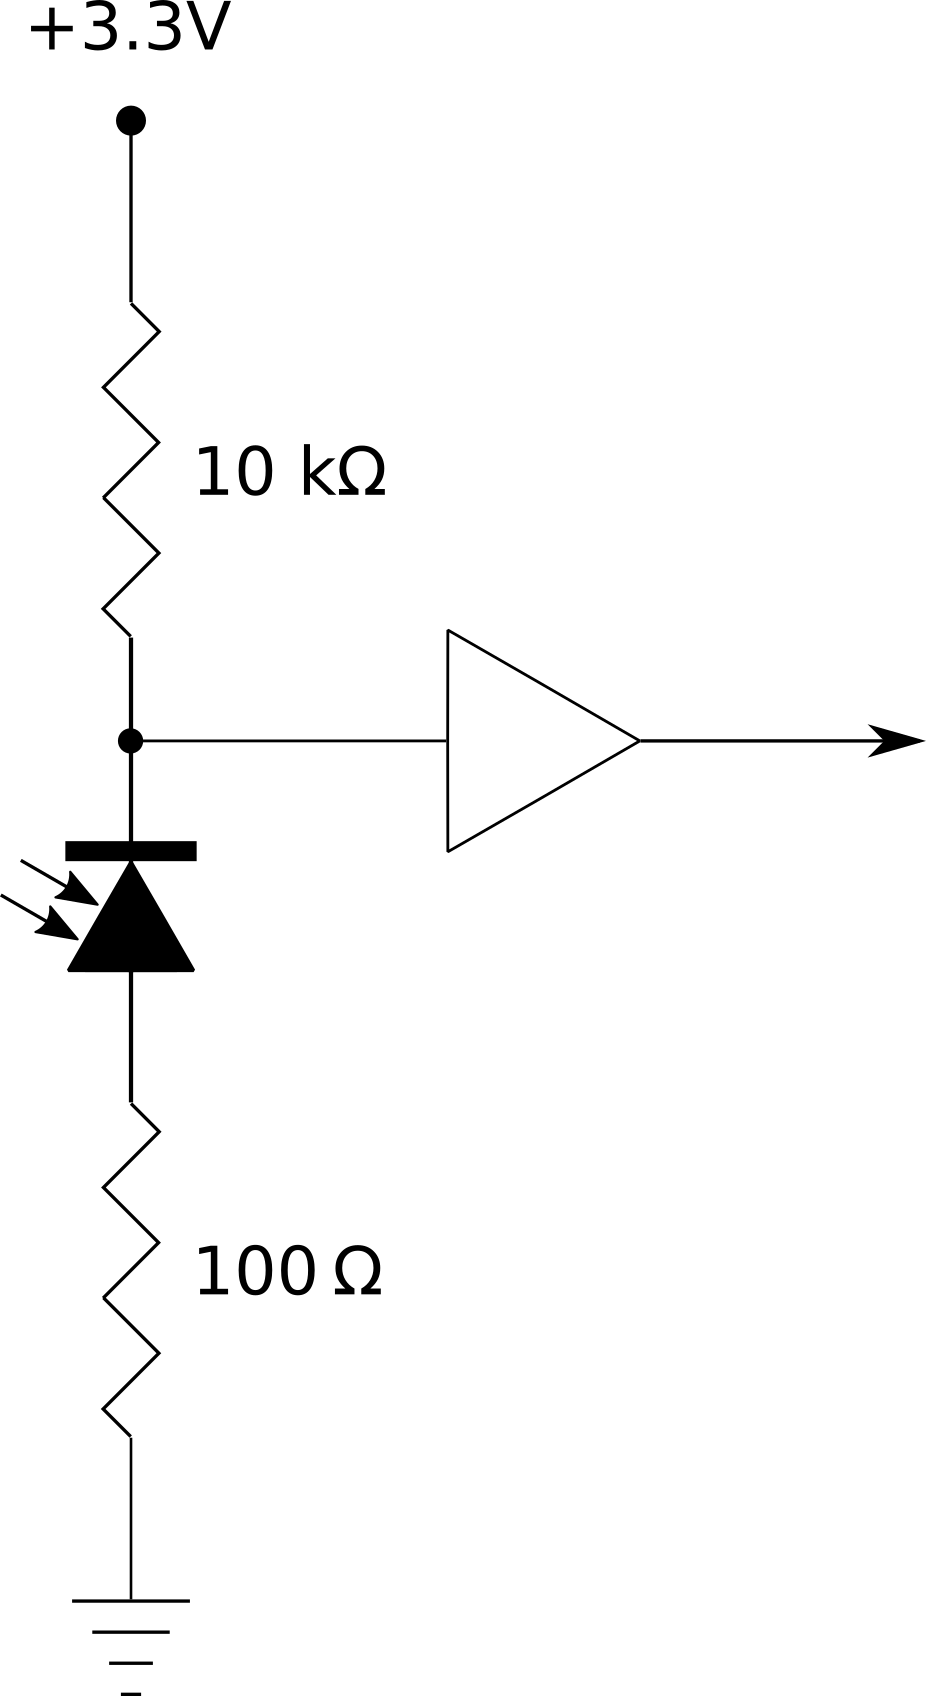
\includegraphics[height=2in]{graphics/photodiode_pullup_and_GPIO_protection.png}
	\caption{The photodiode circuit is purposely made as simple as possible
        for transparency of implementation; the \SI{10}{\kilo\ohm} pull-up
        resistor for reliability together with a \SI{100}{\ohm} series
        resistor to protect a bidirectional driver (here represented by a
        generic buffer) from being shorted to ground in case it were
        accidentally set to output a HIGH logic level at the same time the
        photodiode is illuminated.}
	\label{figure:photodiode_pullup}
\end{figure}

The receiver side of the circuit is shown in Figure
\ref{figure:photodiode_pullup}. The photodiode operates in reverse bias
(photoconductive) mode for two reasons: speed, and simplicity of
implementation. The same photodiode operated in photovoltaic mode would be
more sensitive to very low level signals and have a lower dark current, but
would require a transimpedance amplifier for current-to-voltage conversion,
which would make the design more complicated and thereby more difficult to
evaluate for security.

The rest of the design is equally unconventional (Figure
\ref{figure:deep_pipeline}). Rather than using available `IP' blocks
(Intellectual Property---pre-designed software modules delivering standard
functionality such as ARM cores or Ethernet MAC), we prefer a clean-room
design approach built up from IEEE 802.3 standards using semi-formal methods,
avoiding closed-source IP. The result, we believe, in combination with open
tests, will be considered trustworthy by everyone in the world.

\subsection{Design discussion}

Simplicity of implementation is paramount. There are no amplifiers, no MAC
or PHY chips, no process nodes that cannot be de-capped and have a
representative sample to be examined under a microscope. The development tool
chain must be open source and international.

It must be acknowledged that optical TEMPEST, ironically, is a vulnerability
that can be exacerbated by extreme reliance on simplicity of implementation.
But experience with optical TEMPEST and side channels has inspired so many
other researchers to find and exploit diverse vulnerabilities, that the only
remaining avenue of approach is to strike as many components as possible from
the system, in the belief that a component that is not there cannot fail, has
no vulnerabilities, and lasts forever.

% This is a two-column figure.
\begin{figure*}[!t]
    \centering
	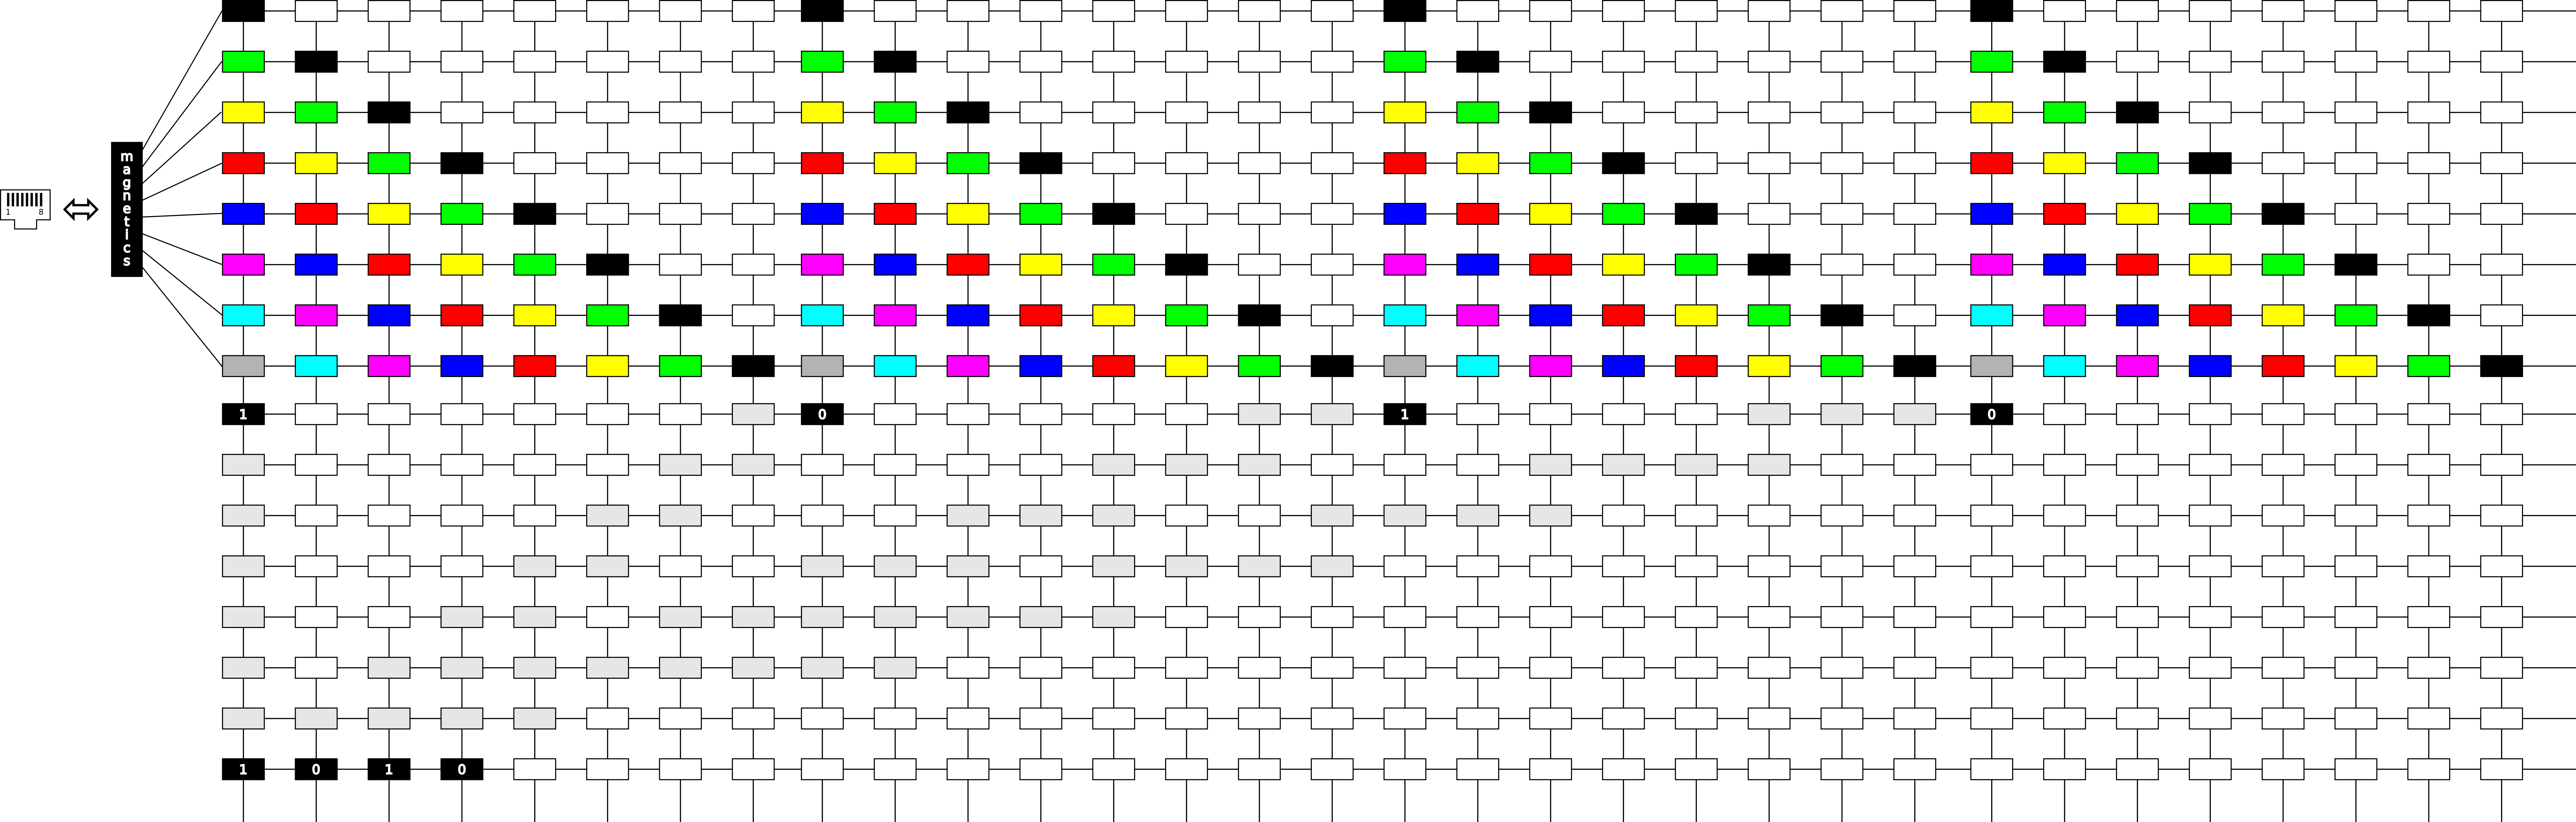
\includegraphics[width=\textwidth]{graphics/deep_pipeline.png}
	\caption{Deep pipeline implementation of an Ethernet MAC; only a small
        portion of the pipeline is shown. The MII is clocked asynchronously
        by the state machine as bits are de-marshalled efficiently into one
        slot each. Profligate expenditure of resources trades off for very
        favourable parallelism and equally transparent computation of sizes,
        offsets, padding, checksum, and digital signature application and
        validation.}
	\label{figure:deep_pipeline}
\end{figure*}

\begin{comment}
Risk of acoustic information leakage from acousto-optic modulator or MMD
modulator. Cooling fan speed modulation acoustic information leakage risk.
Light-tight design. RF, acoustic, vibration, temperature, ELF, power line
conducted emissions: see lit.\ survey in recent papers for a comprehensive
list.

To be honest, I have reservations about the lack of galvanic isolation
through the metal of this component.

\section{Energy Gapping}

Cite the `energy gap' principles from Clive Robinson.

Conductive tape on the seams and for isolation between high side and low side
inside.
\end{comment}

\section{Conclusion}

Since the publication in 2002 of the first peer-reviewed research on
compromising optical emanations, other researchers have carried it further.
But technological progress has shifted the boundaries of what was possible,
necessitating re-visit of the same vulnerabilities from time to time. This is
a general principle of security; vulnerabilities, once fixed, sometimes do
not stay fixed.

\section*{Acknowledgements}

Thanks to many anonymous and pseudonymous commenters on Hacker News
\URL{news.ycombinator.com} for helping develop the ideas in this paper.

% trigger a \newpage just before the given reference
% number - used to balance the columns on the last page
% adjust value as needed - may need to be readjusted if
% the document is modified later

\IEEEtriggeratref{33}

% The "triggered" command can be changed if desired:
%\IEEEtriggercmd{\enlargethispage{-5in}}

\bibliographystyle{IEEEtran}
% argument is your BibTeX string definitions and bibliography database(s)
\bibliography{IEEEabrv,consolidated_bibtex_file}

\end{document}

